\chapter{TiDAL: Visualizing Gene Regulatory Networks}

\section{Purpose}


\section{Motivation}
\subsection{Pathogens act through temporal regulatory cascades}
\subsection{High throughput data combined with computational methods may be used to infer transcription networks}

\begin{figure}
  \centering
  \includegraphics[width=\textwidth,page=17,trim=0.37cm .65cm 0.37cm 0.3cm, clip=true]{images/Figures.pdf}
  \caption{TiDAL interface.}
  \label{Figure:tidal-landing}
\end{figure}

\begin{figure}
  \centering
  \begin{subfigure}[t]{0.3\textwidth}
    \includegraphics[width=\textwidth,page=18,trim=8.5cm 0cm 9cm 0cm, clip=true]{images/Figures.pdf}
    \caption{}
    \label{Figure:tidal-output-heatmap}
  \end{subfigure}
  \begin{subfigure}[t]{.66\textwidth}
    \includegraphics[width=\textwidth,page=19]{images/Figures.pdf}
    \caption{}
    \label{Figure:tidal-output-table}
  \end{subfigure}
  \begin{subfigure}[b]{\textwidth}
    \includegraphics[width=\textwidth,page=20,trim=0.37cm .65cm 0.37cm 0.3cm, clip=true]{images/Figures.pdf}
    \caption{}
    \label{Figure:tidal-output-graphene}
  \end{subfigure}
  \caption{}
  \label{Figure:tidal-output}
\end{figure}

\autocite{zaslavsky2013reconstruction}
\subsection{Temporal regulatory cascades are high dimensional and benefits from visualization}


\section{Solution}
\subsection{Native HTML5 visualizations of TIDAL output}
\subsection{Bind layout styles to visualize high dimensional data}
\subsection{User interaction for exploring network}
Hovering

\section{Implementation}
\subsection{Graphene based web component}
\subsection{Data and layout controllers}
\subsection{Event handling}
